\hypertarget{Rcpp_8cpp}{
\section{src/Rcpp.cpp File Reference}
\label{Rcpp_8cpp}\index{src/Rcpp.cpp@{src/Rcpp.cpp}}
}
{\tt \#include \char`\"{}Rcpp.h\char`\"{}}\par
{\tt \#include $<$cstring$>$}\par


Include dependency graph for Rcpp.cpp:\nopagebreak
\begin{figure}[H]
\begin{center}
\leavevmode
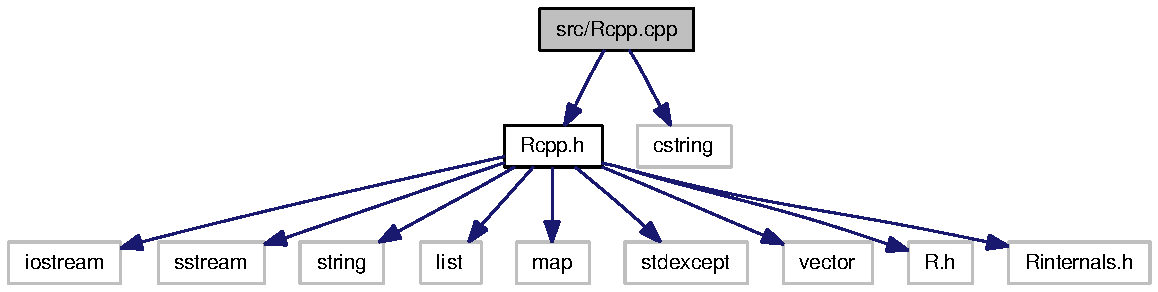
\includegraphics[width=296pt]{Rcpp_8cpp__incl}
\end{center}
\end{figure}
\subsection*{Functions}
\begin{CompactItemize}
\item 
std::ostream \& \hyperlink{Rcpp_8cpp_62c075d47528a48e5fb57c1855c4d71c}{operator$<$$<$} (std::ostream \&os, const \hyperlink{classRcppDate}{RcppDate} \&date)
\item 
\hyperlink{classRcppDate}{RcppDate} \hyperlink{Rcpp_8cpp_dd881a27c2b8e36897a59bca1d04585f}{operator+} (const \hyperlink{classRcppDate}{RcppDate} \&date, int offset)
\item 
int \hyperlink{Rcpp_8cpp_e4e7644b1347f6ac24f818357bbe440d}{operator-} (const \hyperlink{classRcppDate}{RcppDate} \&date2, const \hyperlink{classRcppDate}{RcppDate} \&date1)
\item 
bool \hyperlink{Rcpp_8cpp_f852d3a1ad52776201f385be5ea18c71}{operator$<$} (const \hyperlink{classRcppDate}{RcppDate} \&date1, const \hyperlink{classRcppDate}{RcppDate} \&date2)
\item 
bool \hyperlink{Rcpp_8cpp_80164a177c098301c1d509fdab702567}{operator$>$} (const \hyperlink{classRcppDate}{RcppDate} \&date1, const \hyperlink{classRcppDate}{RcppDate} \&date2)
\item 
bool \hyperlink{Rcpp_8cpp_f7a217e1f5d4a91e2d86fc4da858a6c2}{operator$>$=} (const \hyperlink{classRcppDate}{RcppDate} \&date1, const \hyperlink{classRcppDate}{RcppDate} \&date2)
\item 
bool \hyperlink{Rcpp_8cpp_594132f5ef49b4f477d32289ced4df83}{operator$<$=} (const \hyperlink{classRcppDate}{RcppDate} \&date1, const \hyperlink{classRcppDate}{RcppDate} \&date2)
\item 
bool \hyperlink{Rcpp_8cpp_d6c1518c6eb9480665f532dbcc6dd2d5}{operator==} (const \hyperlink{classRcppDate}{RcppDate} \&date1, const \hyperlink{classRcppDate}{RcppDate} \&date2)
\item 
char $\ast$ \hyperlink{Rcpp_8cpp_86330168f60698ba4d745bb97cdbb15b}{copyMessageToR} (const char $\ast$const mesg)
\end{CompactItemize}


\subsection{Function Documentation}
\hypertarget{Rcpp_8cpp_86330168f60698ba4d745bb97cdbb15b}{
\index{Rcpp.cpp@{Rcpp.cpp}!copyMessageToR@{copyMessageToR}}
\index{copyMessageToR@{copyMessageToR}!Rcpp.cpp@{Rcpp.cpp}}
\subsubsection[{copyMessageToR}]{\setlength{\rightskip}{0pt plus 5cm}char$\ast$ copyMessageToR (const char $\ast$const  {\em mesg})}}
\label{Rcpp_8cpp_86330168f60698ba4d745bb97cdbb15b}




Definition at line 995 of file Rcpp.cpp.

Referenced by Rcpp\_\-Example(), RcppDateExample(), RcppParamsExample(), and RcppVectorExample().\hypertarget{Rcpp_8cpp_dd881a27c2b8e36897a59bca1d04585f}{
\index{Rcpp.cpp@{Rcpp.cpp}!operator+@{operator+}}
\index{operator+@{operator+}!Rcpp.cpp@{Rcpp.cpp}}
\subsubsection[{operator+}]{\setlength{\rightskip}{0pt plus 5cm}{\bf RcppDate} operator+ (const {\bf RcppDate} \& {\em date}, \/  int {\em offset})}}
\label{Rcpp_8cpp_dd881a27c2b8e36897a59bca1d04585f}




Definition at line 805 of file Rcpp.cpp.

References RcppDate::day, RcppDate::jdn, RcppDate::jdn2mdy(), RcppDate::month, and RcppDate::year.

Here is the call graph for this function:\nopagebreak
\begin{figure}[H]
\begin{center}
\leavevmode
\includegraphics[width=120pt]{Rcpp_8cpp_dd881a27c2b8e36897a59bca1d04585f_cgraph}
\end{center}
\end{figure}
\hypertarget{Rcpp_8cpp_e4e7644b1347f6ac24f818357bbe440d}{
\index{Rcpp.cpp@{Rcpp.cpp}!operator-@{operator-}}
\index{operator-@{operator-}!Rcpp.cpp@{Rcpp.cpp}}
\subsubsection[{operator-}]{\setlength{\rightskip}{0pt plus 5cm}int operator- (const {\bf RcppDate} \& {\em date2}, \/  const {\bf RcppDate} \& {\em date1})}}
\label{Rcpp_8cpp_e4e7644b1347f6ac24f818357bbe440d}




Definition at line 812 of file Rcpp.cpp.

References RcppDate::jdn.\hypertarget{Rcpp_8cpp_f852d3a1ad52776201f385be5ea18c71}{
\index{Rcpp.cpp@{Rcpp.cpp}!operator$<$@{operator$<$}}
\index{operator$<$@{operator$<$}!Rcpp.cpp@{Rcpp.cpp}}
\subsubsection[{operator$<$}]{\setlength{\rightskip}{0pt plus 5cm}bool operator$<$ (const {\bf RcppDate} \& {\em date1}, \/  const {\bf RcppDate} \& {\em date2})}}
\label{Rcpp_8cpp_f852d3a1ad52776201f385be5ea18c71}




Definition at line 816 of file Rcpp.cpp.

References RcppDate::jdn.\hypertarget{Rcpp_8cpp_62c075d47528a48e5fb57c1855c4d71c}{
\index{Rcpp.cpp@{Rcpp.cpp}!operator$<$$<$@{operator$<$$<$}}
\index{operator$<$$<$@{operator$<$$<$}!Rcpp.cpp@{Rcpp.cpp}}
\subsubsection[{operator$<$$<$}]{\setlength{\rightskip}{0pt plus 5cm}std::ostream\& operator$<$$<$ (std::ostream \& {\em os}, \/  const {\bf RcppDate} \& {\em date})}}
\label{Rcpp_8cpp_62c075d47528a48e5fb57c1855c4d71c}




Definition at line 799 of file Rcpp.cpp.

References RcppDate::getDay(), RcppDate::getMonth(), and RcppDate::getYear().

Here is the call graph for this function:\nopagebreak
\begin{figure}[H]
\begin{center}
\leavevmode
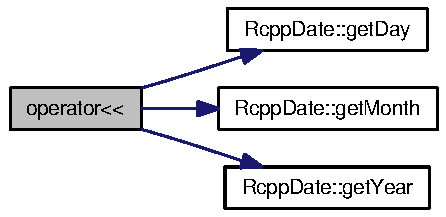
\includegraphics[width=125pt]{Rcpp_8cpp_62c075d47528a48e5fb57c1855c4d71c_cgraph}
\end{center}
\end{figure}
\hypertarget{Rcpp_8cpp_594132f5ef49b4f477d32289ced4df83}{
\index{Rcpp.cpp@{Rcpp.cpp}!operator$<$=@{operator$<$=}}
\index{operator$<$=@{operator$<$=}!Rcpp.cpp@{Rcpp.cpp}}
\subsubsection[{operator$<$=}]{\setlength{\rightskip}{0pt plus 5cm}bool operator$<$= (const {\bf RcppDate} \& {\em date1}, \/  const {\bf RcppDate} \& {\em date2})}}
\label{Rcpp_8cpp_594132f5ef49b4f477d32289ced4df83}




Definition at line 828 of file Rcpp.cpp.

References RcppDate::jdn.\hypertarget{Rcpp_8cpp_d6c1518c6eb9480665f532dbcc6dd2d5}{
\index{Rcpp.cpp@{Rcpp.cpp}!operator==@{operator==}}
\index{operator==@{operator==}!Rcpp.cpp@{Rcpp.cpp}}
\subsubsection[{operator==}]{\setlength{\rightskip}{0pt plus 5cm}bool operator== (const {\bf RcppDate} \& {\em date1}, \/  const {\bf RcppDate} \& {\em date2})}}
\label{Rcpp_8cpp_d6c1518c6eb9480665f532dbcc6dd2d5}




Definition at line 832 of file Rcpp.cpp.

References RcppDate::jdn.\hypertarget{Rcpp_8cpp_80164a177c098301c1d509fdab702567}{
\index{Rcpp.cpp@{Rcpp.cpp}!operator$>$@{operator$>$}}
\index{operator$>$@{operator$>$}!Rcpp.cpp@{Rcpp.cpp}}
\subsubsection[{operator$>$}]{\setlength{\rightskip}{0pt plus 5cm}bool operator$>$ (const {\bf RcppDate} \& {\em date1}, \/  const {\bf RcppDate} \& {\em date2})}}
\label{Rcpp_8cpp_80164a177c098301c1d509fdab702567}




Definition at line 820 of file Rcpp.cpp.

References RcppDate::jdn.\hypertarget{Rcpp_8cpp_f7a217e1f5d4a91e2d86fc4da858a6c2}{
\index{Rcpp.cpp@{Rcpp.cpp}!operator$>$=@{operator$>$=}}
\index{operator$>$=@{operator$>$=}!Rcpp.cpp@{Rcpp.cpp}}
\subsubsection[{operator$>$=}]{\setlength{\rightskip}{0pt plus 5cm}bool operator$>$= (const {\bf RcppDate} \& {\em date1}, \/  const {\bf RcppDate} \& {\em date2})}}
\label{Rcpp_8cpp_f7a217e1f5d4a91e2d86fc4da858a6c2}




Definition at line 824 of file Rcpp.cpp.

References RcppDate::jdn.